%%%%%%%%%%%%%%%%%%%%%%%%%%%%%%%%%%%%%%%%%%%%%%%%%%%%%%%%%%%%%%%%%%%%%%%%%%%%%%%%%%%%%%%%%
% Section 5: Xilinx Designs
%	This section contains a description of the following:
%	- Vivado FPGA designs and netlists (with terminology)
%	- Design data structures in RapidSmith, 
%	- Cell Libraries and how to generate new cell libraries  
%%%%%%%%%%%%%%%%%%%%%%%%%%%%%%%%%%%%%%%%%%%%%%%%%%%%%%%%%%%%%%%%%%%%%%%%%%%%%%%%%%%%%%%%%
\newpage
\section{Designs}

\subsection{Xilinx Netlists} \label{sec:xilinxNetlist}
During the synthesis stage of implementation, a digital circuit expressed using
RTL (VHDL or Verilog) is translated to a lower level Xilinx netlist. This
netlist describes a digital circuit in terms of primitive elements that can
directly target hardware on a Xilinx FPGA. In terms of granularity, a Xilinx
netlist is more abstract than gates and transistors, but more detailed than RTL. A list of valid
primitives (also called \cls{Cell}s) that can be used within a Xilinx netlist
can be found
\href{http://www.xilinx.com/support/documentation/sw_manuals/xilinx2016_2/ug953-vivado-7series-libraries.pdf}{\color{blue}{here}}
for 7 Series devices and
\href{http://www.xilinx.com/support/documentation/sw_manuals/xilinx2014_1/ug974-vivado-ultrascale-libraries.pdf}{\color{blue}{here}}
for Ultrascale devices. It is suggested that users of RapidSmith become
familiar with the primitives found in these documents, and how they are used.
The primitives of a Xilinx netlist are wired together to create a digital
circuit (such as an 32-bit adder) capable of being implemented on an FPGA.
\autoref{fig:schematic} shows an example netlist of a 3-bit counter that has
been synthesized in Vivado. 

\begin{figure}[H]
 \centering
 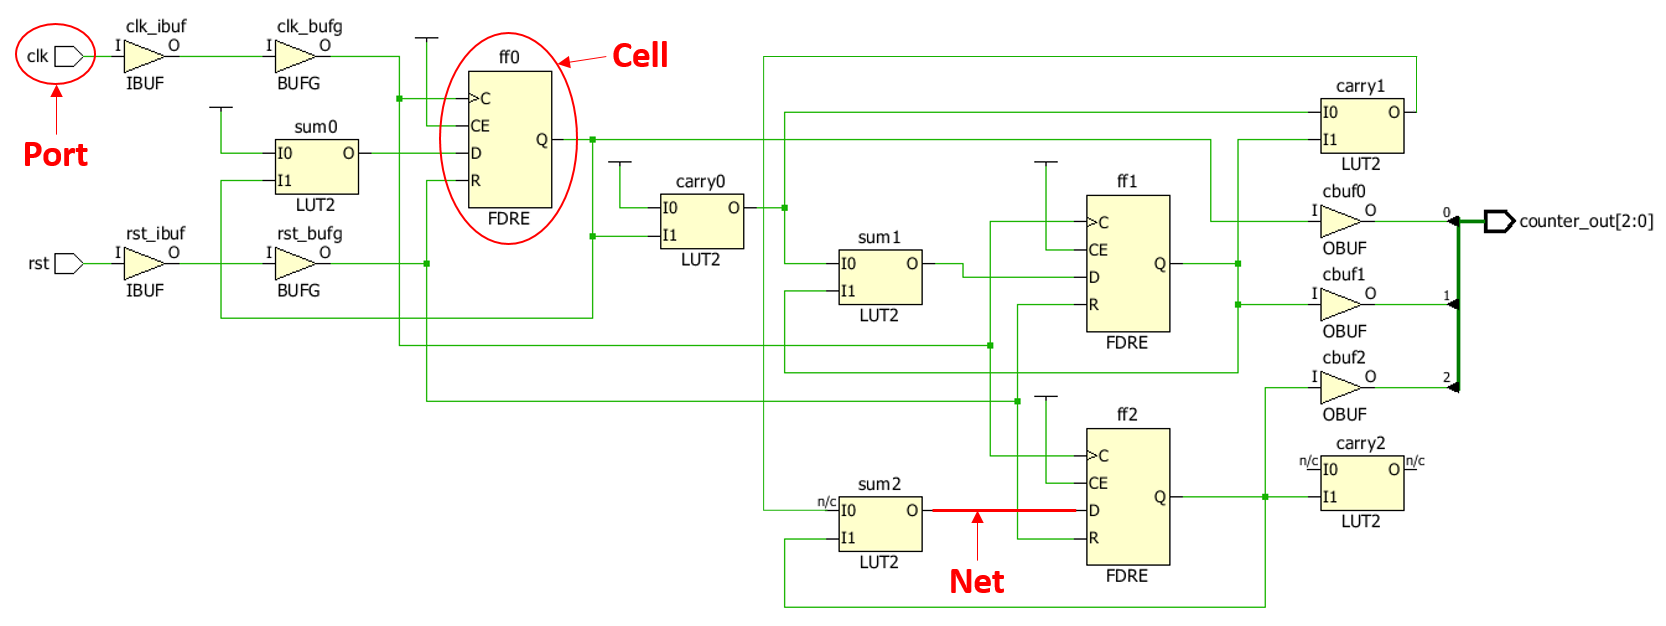
\includegraphics[width=1\columnwidth]{schematic.png}
 \caption{Schematic of a 3-bit counter in Vivado using LUT and FDRE cells.
 The yellow boxes are \cls{Cell}s, the green lines are \cls{Net}s, and and the
 white figures on the edge of the diagram are \cls{Port}s. An example of each
 of these netlist components have been highlighted.}
 \label{fig:schematic}
\end{figure}

As the figure shows, Vivado netlists are composed of three primary components:
\cls{Cell}s, \cls{Net}s, and \cls{Port}s. \cls{Cell}s are \pgm{instances} of
Xilinx primitives. They are the basic building blocks of a Xilinx netlist and
implement the actual logic of a digital design. The most commonly used
\cls{Cell}s include:

\begin{itemize}
  \item \pgm{Look Up Tables} (LUTs): Implement logic equations such as
  $O6 = (A1 + A2) \oplus A3$.
  \item \pgm{Flip Flops} (FDxx): Single-bit storage elements.
  \autoref{fig:schematic} uses an FDRE cell which specifies a rising-edge
  Flip Flop with a reset port, but ties the clock enable port high. Other
  types of FDxx cells can be used to include a clock enable signal (replace xx
  with the corresponding letters).
  \item \pgm{Block Ram} (BRAMs): On-chip FPGA memory cell.
  \item \pgm{Digital Signal Processing Units} (DSPs): Perform complex arithmetic
  functions efficiently.
  \item \pgm{Buffers} (BUF): IO, clock, and other types of signal buffers. 
\end{itemize}

\noindent
There exists several other types of \cls{Cell}s, but the ones in the list above
are the most prevalent. \cls{Net}s are used to connect \cls{Cell}s together. In
other words, the output of one \cls{Cell} is wired to the input of another
\cls{Cell} using a \cls{Net}. \cls{Port}s are simply design
Input/Output (IO). In terms of an FPGA design, \cls{Port}s are connected to
specific peripheral pins of the FPGA for chip IO. It is important to note that
a Xilinx netlist is purely logical, there is no physical information within the
netlist (i.e. there is not information about where the \cls{Cell}s have been
placed, or how the \cls{Net}s have been routed). When exporting a design from
Vivado, the Xilinx netlist representation is converted to EDIF. In order to
recreate the design in RapidSmith, the EDIF file is parsed and converted to a
custom netlist structure described in the next section.

\subsection {RS2 Netlist Data Structures} \label{sec:designDS}

RapidSmith netlists are modeled closely after Xilinx netlists. In fact,
much of the terminology between the two are identical or very similar. For those
that are familiar with Vivado designs, this should make the transition to
RapidSmith straightforward. The data structures that constitute a RapidSmith
netlist can be found in the package \pkg{byu.edu.ece.rapidSmith.design.subsite}.
The package hierarchy can be seen in \autoref{fig:designDS}.

\begin{figure}[H]
 \centering
 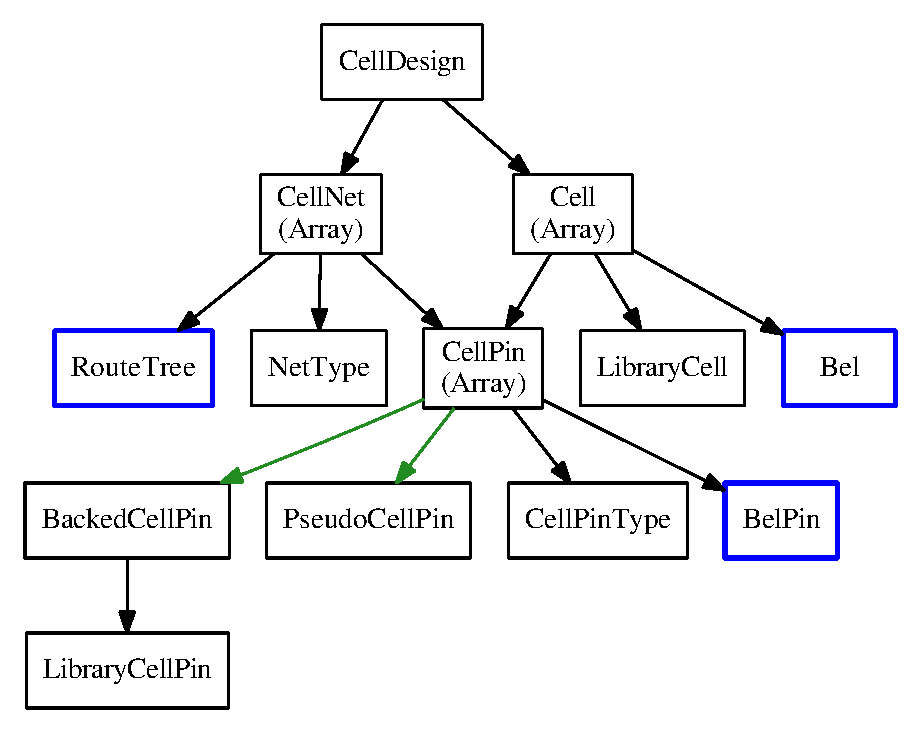
\includegraphics[width=.6\columnwidth]{designDS.eps}
 \caption{RapidSmith 2 design data structure tree. Black arrows represent
 composition (i.e. a \cls{CellDesign} contains an array of \cls{CellNet}s and
 an array of \cls{Cell}s). Green arrows represent inheritance (i.e. a
 \cls{CellPin} can be either a \cls{BackedCellPin} or a
 \cls{PseudoCellPin}). Blue boxes represent physical implementation components
 of the netlist (i.e. what physical \cls{Bel} a \cls{Cell} is placed on, or what
 physical \cls{Wire}s are used in a \cls{CellNet}).}
 \label{fig:designDS}
\end{figure}

\noindent
A \cls{CellDesign} is the top level design object in RapidSmith. It consists of
a collection of \cls{Cell} objects, interconnected by \cls{CellNet}s. RapidSmith
\cls{Cell}s are equivalent to Xilinx \cls{Cell}s and RapidSmith \cls{CellNet}s
are equivalent to Xilinx \cls{Net}s. \cls{Cell} objects have a template
\cls{LibraryCell}, which represents a Xilinx primitive. They also have a
collection of \cls{CellPin}s, which can be thought of as \cls{Cell} IO. 
During the placement phase of implementation, \cls{Cell}s may be mapped onto
\cls{BEL}s and the corresponding \cls{CellPin}s mapped onto \cls{BelPin}s.
Placement is described in more detail in \autoref{sec:placement}. \cls{CellNet}
objects connect \cls{Cell}s together via their \cls{CellPin}s.
During the routing phase of implementation, a \cls{CellNet} maps onto one or
more \cls{RouteTree}s. Routing is described in more detail in
\autoref{sec:routing}. The best way to learn how to use these classes is to read
through the \href{https://github.com/byuccl/RapidSmith2}{\color{blue}{Javadocs}}, but
important aspects of each class is included in the following subsections.


\subsubsection{\cls{CellDesign}}
As previously mentioned, the \cls{CellDesign} class is the top level netlist
structure. A Vivado design is converted from a Tincr checkpoint to a
\cls{CellDesign} on import, and converted from a \cls{CellDesign} to a Tincr
checkpoint on design export. It contains the following:

\begin{itemize}
  \item A list of uniquely named \cls{Cell}s in the design.
  \item A list of uniquely named \cls{CellNet}s in the design
  \item Global GND and VCC \cls{CellNet}s
  \item \cls{Cell} placement information (where each cell is placed)
  \item Internal routing configuration for each \pgm{used} \cls {Site} (in the
  form of \cls{Site} \cls{PIP}s)
  \item A list of XDC constraints imported from Vivado. See \autoref{sec:import}
  for more information about XDC constraints and how they are represented in
  RapidSmith.
\end{itemize}

\noindent
The \cls{CellDesign} class has a variety of methods to retrieve and manipulate
the \cls{Cell}s and \cls{CellNet}s of a design, place \cls{Cell}s onto
physical \cls{BEL}s, configure sub-site routing, and perform several other
tasks. See the
\href{https://github.com/byuccl/RapidSmith2}{\color{blue}{Javadocs}} for the
exact API.
 
\subsubsection{\cls{Cell}}
This section contains a few things you should know about \cls{Cell}s in, no
particular order.

\begin {itemize}
  \item A \cls{Cell} always contains a reference to a backing \cls{LibraryCell}.
  A \cls{LibraryCell} is equivalent to a Xilinx primitive cell (described in
  \autoref{sec:xilinxNetlist}), and serves as a template for instantiated
  \cls{Cell} objects. The template is used to save memory when creating several
  \cls{Cell}s of the same type. Whenever a new \cls{Cell} object is created, a
  corresponding \cls{LibraryCell} must be specified in the constructor.
  \autoref{code:cells} demonstrates how to create a new cell in RapidSmith and
  filter cells based on their type.
  
\begin{lstlisting}[caption=How to create new cells in RapidSmith,
label=code:cells] 
// You need to have a cell library to create a cell
CellLibrary libCells = new CellLibrary(RSEnvironment.defaultEnv()
				.getPartFolderPath("xc7a100t-csg324")
				.resolve("cell_library.xml"));

// How to create a new cell. The first argument is the name of the cell, the
// second argument is the library cell
Cell cell = new Cell("myCell", libCells.get("LUT6"));

// Get all cells in a design of a certain type
CellDesign design = getCellDesign();
Stream<Cell> cells = design.getCellsOfType(libCells.get("FDRE"));
\end{lstlisting}

  The method call \texttt{CellDesign.getCellsOfType(String,CellLibrary)} can be
  used to get all \cls{Cell}s in the current design with a specific
  \cls{LibraryCell} type.
  
  \item A \cls{Cell} has a list of \cls{CellPin}s that can connect to
  \cls{CellNet}s. The methods \texttt{Cell.getPins()},
  \texttt{Cell.getInputPins()}, and \texttt{Cell.getOutputPins()} can be used to
  get a handle to the pins of a \cls{Cell}. If more pins are
  needed on a \cls{Cell}, \cls{PseudoCellPin} objects can be attached (see
  \autoref{sec:cellPin}). \item \cls{Cell}s can be placed onto \cls{BEL}s of the
  current \cls{Device}. See \autoref{sec:placement} for more information about
  cell placement.
  \item Top-level \cls{Port}s in Vivado (design input/output) are represented as
  Port \cls{Cell}s in RapidSmith. Specifically, there are three types of port cells: IPORT, 
  OPORT, and IOPORT. The method \texttt{CellDesign.getPorts()} can
  be used to iterate through the port \cls{Cell}s in a design, and the method
  \texttt{Cell.isPort()} can be used to determine if a given \cls{Cell} is
  actually a port.
  \item Cells can be MACRO cells or LEAF cells. Leaf cells are the types of
  cells described in \autoref{sec:xilinxNetlist}. Macro cells are described in
  more detail in \autoref{sec:macros}.
\end{itemize}

\subsubsection{\cls{CellPin}} \label{sec:cellPin}

There are two types of \cls{CellPin} objects in RapidSmith:
(1) \cls{BackedCellPin}s and (2) \cls{PseudoCellPin}s. \cls{BackedCellPin}s are
straightforward. They represent a \cls{LibraryCellPin}, which is a pin attached
to the corresponding \cls{LibraryCell} of a \cls{Cell}. These pins are used as
signal input and signal output. On the other hand, \cls{PseudoCellPin}s are
``fake" \cls{CellPin} objects which are added to a \cls{Cell} after
the \cls{Cell} has been created. They don't affect the functionality of the
\cls{Cell}, but are needed for physical implementation. An example of where a
\cls{PseudoCellPin} is needed can be seen in \autoref{fig:pseudoPin}.

\begin{figure}[H]
 \centering
 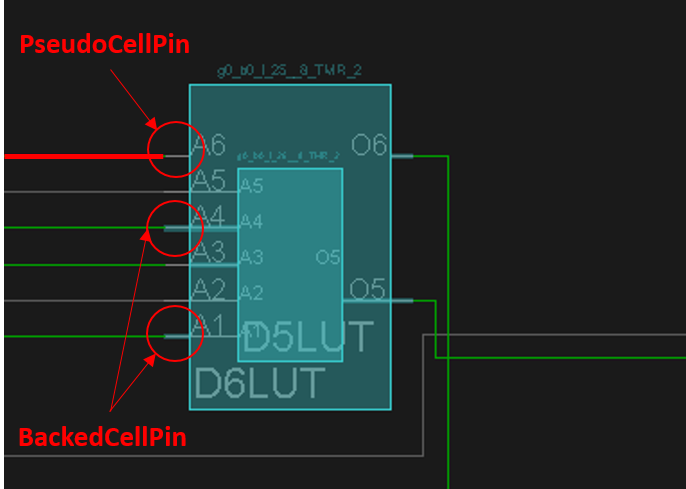
\includegraphics[width=.5\columnwidth]{pseudoPin.png}
 \caption{An example where a \cls{PseudoCellPin} in RapidSmith may be needed.
 Both a \cls{PseudoCellPin} and \cls{BackedCellPin} are pointed out. The red net
 in the image (going into the A6 pin) is the power net (VCC).}
 \label{fig:pseudoPin}
\end{figure}

\noindent
In the figure, a cell of type LUT2 has been placed onto a D6LUT \cls{BEL} of a
SLICEL. The two \cls{CellPin}s of the LUT2 have been mapped to the A1 and A4
pins of the \cls{BEL} (which have been highlighted in blue), connected to
\cls{Net}s, and routed. This is expected behavior based on the netlist.
Also, the global VCC net has been routed to the A6 \cls{BelPin}. This is
necessary due to the hardware implementation of LUTs. However, in the
netlist view of the circuit, the fact that VCC needs to be routed to the A6 pin
is not at all represented (a \cls{CellNet} can only be connected to
\cls{CellPin}s). This is where \cls{PseudoCellPin}s are helpful.
In RapidSmith, a \cls{PseudoCellPin} can be added to the LUT2 cell (called
``VCCPin''), mapped to the A6 \cls{BelPin}, and attached to the global VCC
\cls{CellNet}. This gives a more complete view of how the netlist needs to be
physically implemented. \cls{PseudoCellPin}s are created and added
automatically to \cls{Cell}s when importing a Tincr checkpoint. If you are
creating \cls{Cell}s from scratch, a \cls{PseudoCellPin} can be added with the
method call \texttt{Cell.attachPseudoPin(string,PinDirection)}. To determine if
a \cls{CellPin} is a \cls{PseudoCellPin}, the method call
\texttt{CellPin.isPseudoPin()} can be used. That
being said, in general \pgm{users do not need to worry about the different
between pseudo and backed \cls{CellPin}s} when creating a CAD algorithm. They
function identically, so you can use the higher level handles to the
\cls{CellPin} interface instead.

Each \cls{CellPin} object also has a \cls{CellPinType} and \cls{PinDirection}
enumeration. \autoref{tab:pinEnums} displays the possible values for both of
these enumerations. The \cls{CellPinType} field can be used to find all RESET
\cls{CellPin}s in a design, determine if a \cls{CellNet} is a clock net (it
connects to pins of type CLOCK), and other useful functions. The
\cls{PinDirection} field is typically used to filter a list of \cls{CellPin}s by
their direction. It it especially useful in determining if a pin on a \cls{Cell}
is of type INOUT. 

\begin{table} [h!]
\begin{center}
\begin{tabu}{ |c|l| }
%\begin{tabular}{ |p{2cm}|p{3cm}| }
\hline
\pgm{Enum} & \multicolumn{1}{|c|}{\textbf{Values}}\\
%\pgm{Enum} & \textbf{Values} & \textbf{Description} \\
\hline
\hline
 & CLEAR \\ 
 & CLOCK  \\
 & ENABLE \\      
 & PRESET \\ 
 & RESET \\
\cls{CellPinType} & REUSED \\
 & SET \\
 & SETRESET \\
 & WRITE\_ENABLE \\
 & DATA \\
 & PSEUDO \\
\hline
 & IN \\
\cls{PinDirection} & OUT \\ 
 & INOUT\\ 
\hline
\end{tabu}
\caption{Enumerations for the \cls{CellPin} class}
\label{tab:pinEnums}
\end{center}
\end{table}

\subsubsection{\cls{CellNet}}
\cls{CellNet}s are used to wire components of a logical netlist
together. Specifically, a \cls{CellNet} connects an output
\cls{CellPin} to several input \cls{CellPin}s with the purpose of transferring
a signal from one \cls{Cell} to another. The remainder of this section details
important aspects about \cls{CellNet}s in RapidSmith.

\begin{itemize}
  \item \cls{CellNet}s are routed using the \cls{RouteTree} data structure.
  Routing in RapidSmith is described in more detail in \autoref{sec:routing}.
  \item All \cls{CellNet}s have a \cls{NetType} enumeration. Possible values for
  \cls{NetType} include VCC, GND, and WIRE. VCC is reserved for power nets, GND
  is reserved for ground nets, and WIRE represents all other nets in the design.
  Other \cls{NetType}s could be added to this list in the future (such
  as CLOCK), but for now they are not differentiated.
  \item VCC and GND nets (also called static nets) are treated specially in
  RapidSmith in two ways. (1) Vivado designs can have multiple nets that
  correspond to VCC or GND, but they all logically represent the same thing.
  This representation can be challenging to work with when designing CAD tools.
  RapidSmith takes a different approach. When a design is imported from Vivado,
  all VCC nets are collapsed into a single VCC net that is sourced by a global
  VCC cell (the same applies to GND nets). We have found this representation
  much easier to work with. The function calls \texttt{CellDesign.getVccNet()}
  and \texttt{CellDesign.getGndNet()} can be used to retrieve these special
  nets from the design. If you add a VCC net to a design that already has a VCC
  net, the old net will be overridden. (2) When a static net is routed, it
  doesn't have a single source driving it. Rather, the net is partitioned
  into sections with each section having a single source. In an FPGA, each of
  these sources corresponds to a TIEOFF within a switchbox tile. This is shown
  in \autoref{fig:staticNetSources}.
  
  \begin{figure}[H]
   \centering
   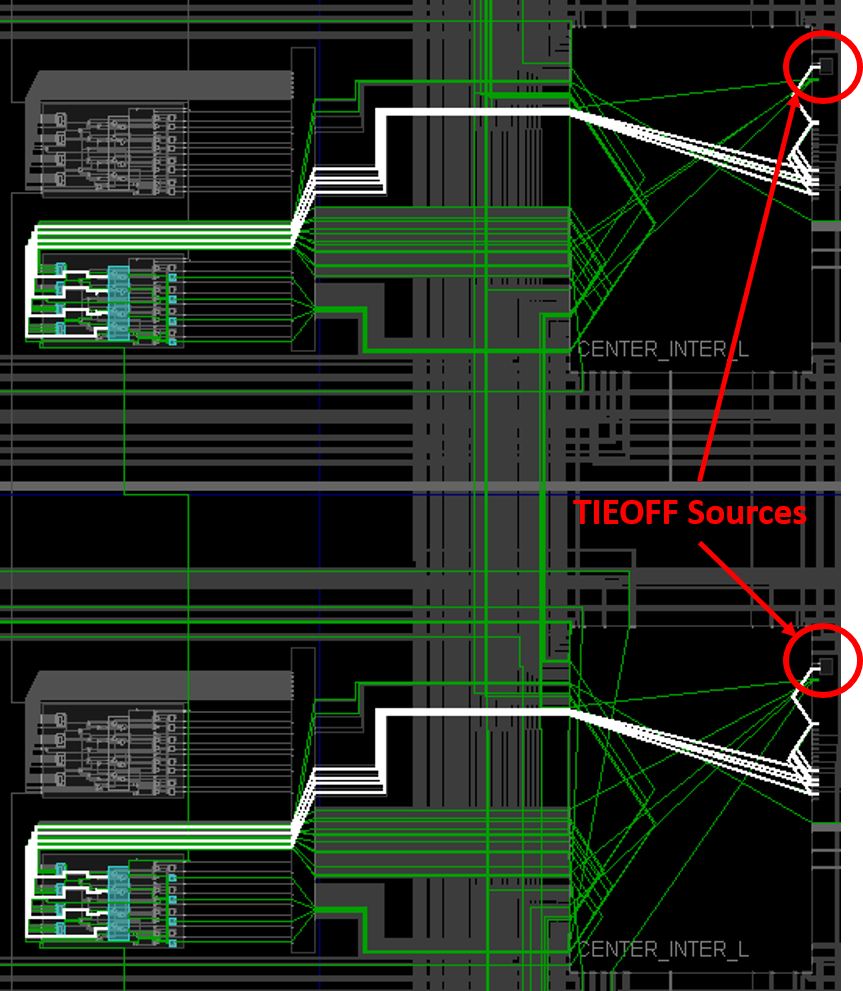
\includegraphics[width=.49\columnwidth]{staticNetSources.png}
   \caption{Static net multiple sources example. The higlighted white wires are
   a part of the same GND net, and the circled red areas are the source TIEOFFs
   for the GND net. In this image, only two sources are shown.}
   \label{fig:staticNetSources}
  \end{figure}
  
  RapidSmith handles this oddity by allowing \cls{CellNet}s to have more than
  one RouteTree object associated with it. In the case of
  \autoref{fig:staticNetSources} the GND net would have two \cls{RouteTree}
  objects associated with it, one for each source TIEOFF.
   
  \item Most \cls{CellNet}s have a single source pin and multiple sink pins
  (referred to as the ``fanout'' of the net). When routing a net that fits
  this description, only one RouteTree needs to be specified. However, there are
  two noticable exceptions to the common case: (1) static nets (described
  in the bullet point above) and (2) nets with multiple drivers (involving IO
  pins). In a Xilinx FPGA, this is most often seen in IOB pads. An example is
  shown in \autoref{fig:iobNet}. The highlighted net can be driven by both the OBUF output, and from an
  external source. RapidSmith 2 supports nets with multiple drivers. The
  function call \texttt{CellNet.getAllSources()} can be used to retrieve all
  possible source \cls{CellPin}s of a net.
  
  \begin{figure}[H]
   \centering
   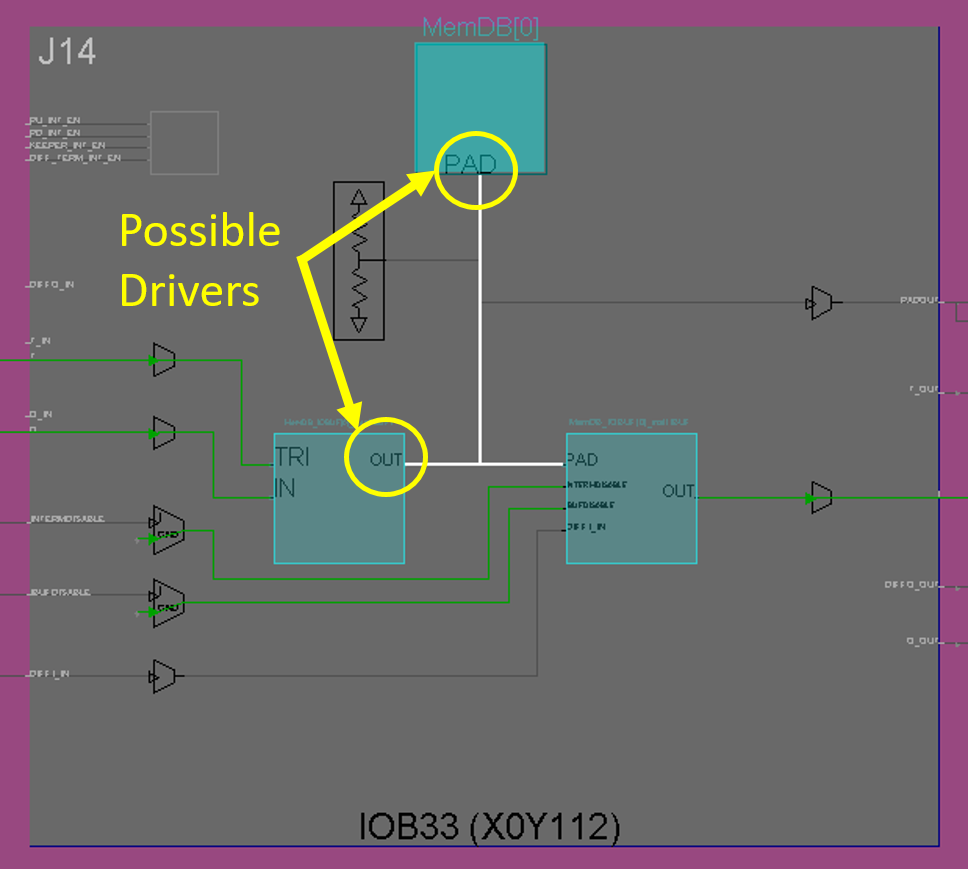
\includegraphics[width=.5\columnwidth]{iobNet.png}
   \caption{An example of net (highlighted in white) that can be driven by more
   than once source.}
   \label{fig:iobNet}
  \end{figure}
  
  \item After a design has been placed, \cls{CellNet}s fall into one of two
  categories: INTRASITE or INTERSITE. \autoref{fig:interVsIntra} shows an
  example of both types of nets. As can be seen, INTRASITE nets do not cross
  \cls{Site} boundaries while INTERSITE nets stretch across multiple
  \cls{Site}s. These types of nets are handled differently during routing. To
  determine if a \cls{CellNet} is an INTRASITE net, the method call
  \texttt{CellNet.isIntrasite()} can be used.
  
  \begin{figure}[H]
   \centering
   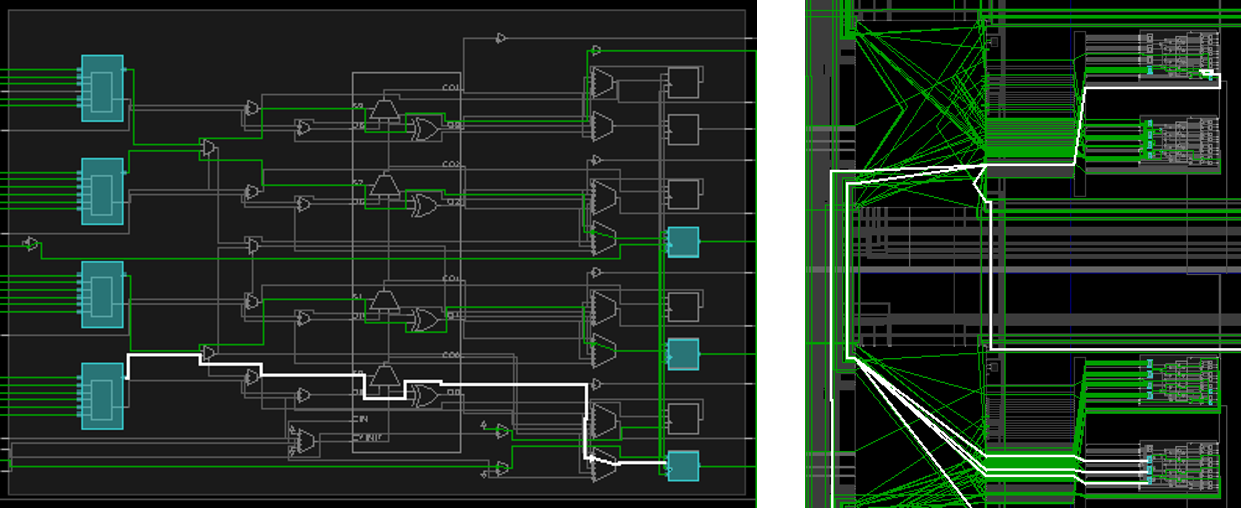
\includegraphics[width=.9\columnwidth]{interVsIntra.png}
   \caption{Example of an INTRASITE net (left) and an INTERSITE net (right).}
   \label{fig:interVsIntra}
  \end{figure}
  
\end{itemize}

\subsubsection{Macro Cells} \label{sec:macros}
Most cells in RapidSmith or Vivado designs are leaf cells (LUTs, Flip Flops,
etc.). However, macro cells can also exist. A macro cell can conceptually be
thought of as a wrapper for related leaf cells. \autoref{fig:macros} shows an
example of an ``IOBUF'' macro cell in Vivado, which is a bidirectional buffer.

\begin{figure}[H]
 \centering
 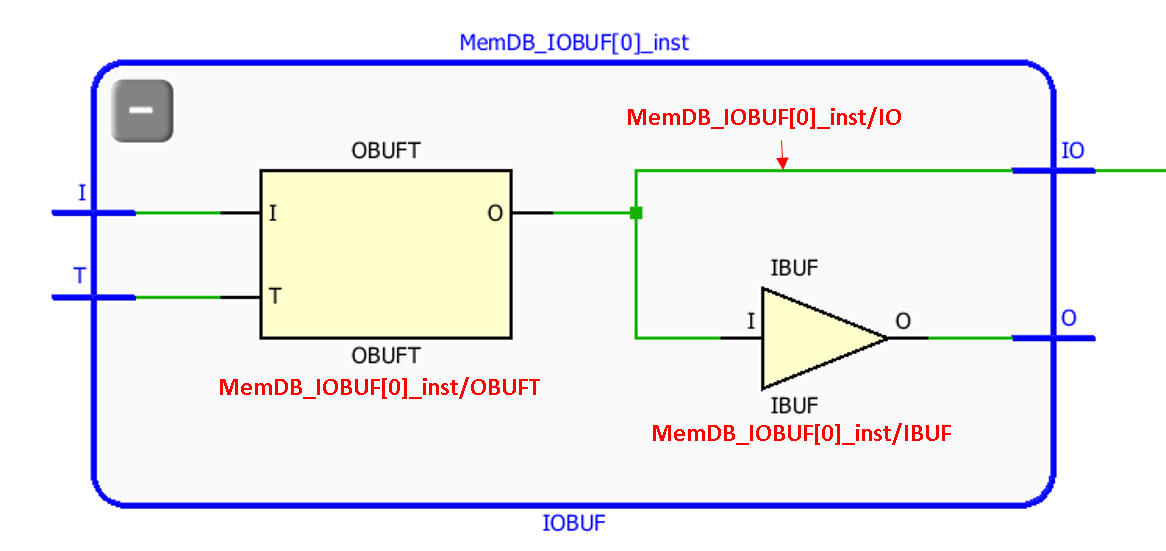
\includegraphics[width=.9\columnwidth]{macro.png}
 \caption{An IOBUF macro in Vivado.}
 \label{fig:macros}
\end{figure}

\noindent 
As the figure shows, the macro consists of two internal cells: one of type
``OBUFT'' and another of type ``IBUF''. The two internal cells are encapsulated
into an external macro cell with the name ``MemDB\_IOBUF[0]\_inst'', and wired
together accordingly. External cell pins of the macro connect to one or more
internal cell pins. Also, internal nets can exist in macros that connect two
internal cells together. RapidSmith now supports importing macro cells from
Vivado and adding them to a \cls{CellDesign}. \autoref{code:macros} gives a
brief introduction to using macro in RapidSmith.

\begin{lstlisting}[caption=How to use macros in RapidSmith,
label=code:macros] 
// Get a handle to a design and cell library
CellDesign design = getCellDesign();
CellLibrary libCells = getCellLibrary();

// Create a new macro cell and add it to a design
Cell macro = new Cell("myMacro", libCells.get("IOBUF"));
design.addCell(macro);

// Connect the macro cell to a net 
CellPin pin = macro.getPin("IO");
design.getNet("TmpNet").connectToPin(pin);

// Iterate through a list of all cells (macro and leaf cells) of a design
for (Cell cell : design.getCells) {
	if ( cell.isMacro() ) {
		List<Cell> internalCells = cell.getInternalCells();
		List<CellNet> internalNets = cell.getInternalNets();
		List<CellPin> externalPins = cell.getPins();
		// do something with the macro info
	}
	else {
		// do something with a regular leaf cell 
	}
}

\end{lstlisting}

\noindent
As the code example above shows, macro cells are generally used
exactly like regular leaf cells. However, there are a few distinctions
between macro cells and leaf cells.

\begin{itemize}
  \item When a macro cell is added to a \cls{CellDesign}, all of the internal
  cells and internal nets are automatically added to the design as well. You do
  not have to worry about adding these yourself. When a macro cell is removed
  from a \cls{CellDesign}, the internal cells and nets are also removed.
  \item When a macro cell pin is connected to a \cellnet, RapidSmith
  automatically connects the net to the corresponding internal pins. When a
  macro cell pin is disconnected from a \cellnet, the internal cell pins are
  disconnected. Nets in RapidSmith only connect to leaf cells (i.e. it is
  essentially a flattened netlist).
  \item Internal cells and nets within a macro cannot be individually added or
  removed from a \cls{CellDesign}. An exception will be thrown if you try to do
  this. Instead, the entire macro cell must be added or removed.
  \item Macros cannot be placed. Rather, the internal cells of a macro should be
  placed instead.
  \item When a \cls{CellDesign} is exported from RapidSmith, macro cells are not
  exported. Only the internal cells and nets are exported and the macro is not
  rebuilt in Vivado.
\end{itemize}

\subsubsection {\cls{PropertyList}}

Most objects in Vivado's Tcl interface have attached properties. These
properties can be used to describe attributes of the object (such as name,
type, etc.), but they can also be used for configuring the object.
\autoref{fig:properties} shows a list of properties for a FDCE flip flop
cell in Vivado.

\begin{figure}[H]
 \centering
 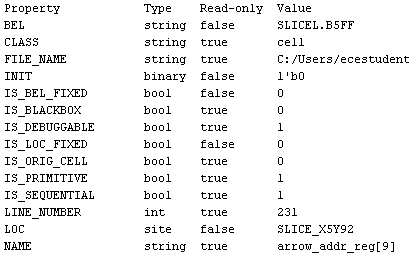
\includegraphics[width=.6\columnwidth]{vivadoProperties.png}
 \caption{Properties of an FDCE cell in Vivado.}
 \label{fig:properties}
\end{figure}

\noindent If you are interested in exploring object properties in
Vivado, the following Tcl command can be used where ``object'' is a cell, bel, or
other Tcl object.

\vspace{-.25cm}
\begin {code}
vivado% report\_\-property \$object
\end{code}

\noindent Cells are the most interesting objects
in terms of properties. This is because the function of a \cls{Cell} is
determined by how it is configured. For example, the memory width of a BRAM cell
in Vivado is configured by setting the ``READ\_WIDTH'' and ``WRITE\_WIDTH''
properties of the cell. Possible values include 1, 2, 4, 9, 18, 36 and 72. The
operation of the BRAM is different depending on how this property is set. Another example is
a D flip flop cell (FDRE) and its ``IS\_C\_INVERTED'' property. This property
indicates if the flip flop will be rising-edge or falling-edge triggered. On
design export, the properties of cells, nets, and the top-level design are
included in the output EDIF netlist of a Tincr Checkpoint (\pgm{if they are not
the default value}).

When RapidSmith parses the EDIF file in a Tincr Checkpoint, the properties
within are stored in a data structure called a \cls{PropertyList}. Each
\cls{CellDesign}, \cls{Cell}, and \cls{CellNet} in RapidSmith has an associated
\cls{PropertyList} object. The \cls{PropertyList} for each \cell in the design
also has a list of default configuration properties. Configuration properties
for \cells are always included in the \cls{PropertyList} even if they are not
explicitly set by the user. As previously stated, this is because the
functionality of the cell is dependent on the values of its configuration
properties. \autoref{code:properties} shows some basic property usage.

\begin{lstlisting}[caption=Using PropertyLists in RapidSmith,
label=code:properties] 
// Create a new FF cell with default properties
CellLibrary libCells = getCellLibrary();
LibraryCell libCell = libCells.get("FDRE");
Cell cell = new Cell("myCell", libCell);

// Get a handle to the cells properties
PropertyList properties = cell.getProperties();

// Print the configurable properties of the cell 
for(String propName : libCell.getConfigurableProperties()) {
	Property prop = properties.get(propName);
	System.out.println(propName + ":");
	System.out.println("\tDefault -> " + prop.getStringValue());
	System.out.println("\tPossible -> " + libCell.getPossibleValues(propName)); 
}

// Iterating over a PropertyList
for (Property prop : properties) {
	System.out.println(prop.getKey() " -> " + prop.getStringValue());
}

// Change the FF to a falling edge flop...this will override the default property 
properties.update("IS_C_INVERTED", PropertyType.EDIF, "1'b1");


\end{lstlisting}

\noindent Here are some additional notes about  cell properties that may be
helpful:

\begin{itemize}
  \item To learn what configuration properties a \cls{Cell} has, open up a
  Vivado design and type the following into the console,
  
  \begin{code}
  Vivado\% link_design -part xc7a100tcsg324-3 -quiet
  Vivado\% set lib_cell [get\_lib\_cells RAMB36E1]
  Vivado\% report_property \$lib_cell 
  \end{code}
  
  replacing ``xc7a100tcsg324-3'' with the part you are using and ``RAMB36E1'' with your
  cell of interest. All properties that start with ``CONFIG'' represent
  configuration properties that a user can set.
  \item Because EDIF properties only support String, Integer, and Boolean types,
  any properties imported from the EDIF file will be one of these types.
  However, from our testing, Vivado always exports its properties as strings.
  \pgm{RapidSmith makes no attempt to parse the Vivado properties into their
  corresponding data structures. All Vivado properties are represented using
  Strings, and it is currently up to the user to parse the properties if they
  need to}.
  \item To learn what configuration properties \pgm{affect the pin mappings of
  a cell}, open the \fil{cellLibrary.xml} file you have, and search for the
  tag ``libcellproperty.'' Pin mappings are described in more detail in
  \autoref{sec:placement}.
  \item Only properties of type \cls{PropertyType.EDIF} will be exported from
  RapidSmith.
  If you create cells in your design and add properties to them, make sure that you
  mark the properties as EDIF properties if you want them to be exported
  All other properties will be ignored during design export.
  \item Some properties not only affect how a \cls{Cell} is configured, but they
  can also affect how a \cls{Site} is configured. For example, on SLICEL
  sites there exists a clock routing mux that chooses between a regular clock
  signal and an inverted signal (\autoref{fig:clkinv}). The output of this
  inverter is connected to all flip flops of the SLICEL, and so decides whether the flip flops are
  all rising-edge or all falling-edge triggered. The clock that is selected is
  decided by the property ``IS\_C\_INVERTED'' of the flip flops cells \pgm{that
  have been placed onto the SLICEL}. The clock inverter is programmed
  automatically based on the cell properties. There are other such properties,
  but they will not be listed here. When creating designs in RapidSmith, it is
  important to not place \cls{Cell}s together that may have conflicting
  properties. RapidSmith does not perform any error checking, and so an error
  in Vivado will be thrown if you violate property restrictions.
  
\begin{figure}[H]
 \centering
 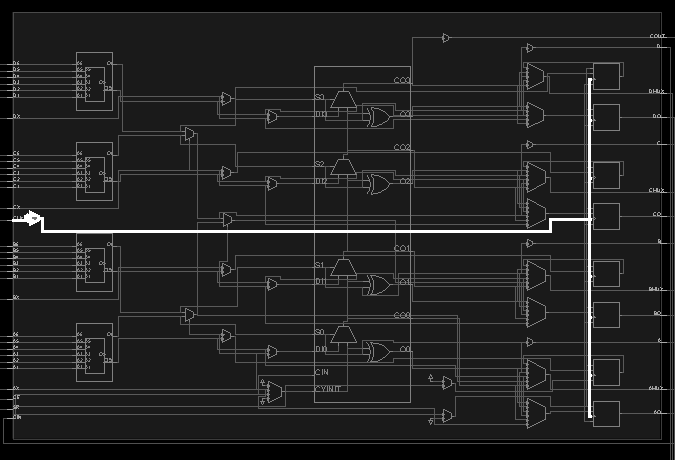
\includegraphics[width=.8\columnwidth]{clkinv.png}
 \caption{A SLICEL clock inverter mux. The highlighted white portion of the
 figure shows the connection of the clock inverter.}
 \label{fig:clkinv}
\end{figure}
  
  
\end{itemize}

\subsection{The Cell Library}

The \cls{CellLibrary} in RapidSmith stores important information about each of
the \cls{LibraryCell}s compatible with a specific Xilinx FPGA part.
This includes: 

\begin {itemize}
  \item The name of the library cell
  \item The name, direction, and type of each library cell pin
  \item Valid placement locations for instances of the library cell
  \item Possible logical-to-physical pin mappings for every library pin
  \item The type of library cell (macro or simple)
  \item Configuration properties of the library cell (TODO)
\end{itemize}

\noindent
When doing any type of netlist modification, the \cls{CellLibrary} is needed.
Currently, each \cls{CellLibrary} corresponds to a specific Xilinx
part.
This means that for each part you use in RapidSmith, a new \cls{CellLibrary}
needs to be generated \footnote{This may change to be family-specific in the
future. Usually, parts in the same family can use the same
\cls{CellLibrary}. The part-specific requirement is very conservative, but is
one that we know is right}.
The rest of this section demonstrates how to get access to a cell library in
RapidSMith, and how to create a new cell library XML file from Tincr.

\subsubsection{Loading a Cell Library}
When a Tincr checkpoint is imported into RapidSmith, a \cls{CellLibrary} is
automatically loaded. To get a handle to the \cls{CellLibrary}, you can use
the method call \texttt{TincrCheckpoint.getLibCells()} on the loaded checkpoint
object. If you don't have a handle to a Tincr Checkpoint, then the cell
library XML can be loaded directly from disk. \autoref{code:cellLibrary}
demonstrates both methods of loading a \cls{CellLibrary}.

\begin{lstlisting}[caption=How to load a CellLibrary,
label=code:cellLibrary] 
// First way, load a Tincr Checkpoint
TincrCheckpoint tcp = VivadoInterface.loadTcp("checkpoint.tcp");
CellLibrary libCells1 = tcp.getLibCells();

// Second way, directly load the cell library from disk
CellLibrary libCells2 = new CellLibrary(RSEnvironment.defaultEnv()
                       .getPartFolderPath("xc7a100t-csg324-3")
                       .resolve("cellLibrary.xml");

\end{lstlisting}

\subsubsection{Adding Custom Macros to a Cell Library} \label{sec:customMacros}
Customized macros can now be added to a \cls{CellLibrary} if desired. This can
be accomplished in two easy steps. 

\begin {enumerate}
  \item Create an XML specification
  of your macro that follows the format laid out below: 

\begin{lstlisting}[language=XML, numbers=none, keywordstyle=, stringstyle=]
<?xml version="1.0" encoding="UTF-8"?>
<root>	
  <macros>    
		<macro>
        <type>RAM128X1D</type>
        <!-- List of internal cells with name and leaf type of each -->
        <cells>
            <internal>
                <name>DP.HIGH</name>
                <type>RAMD64E</type>
            </internal>
            <internal>
                <name>DP.LOW</name>
                <type>RAMD64E</type>
            </internal>
            <internal>
                <name>F7.DP</name>
                <type>MUXF7</type>
            </internal>
			...
        </cells>
        <!-- List of macro pins with name, direction, pin type, and internal connections --> 
        <pins>
            <pin>
                <name>DPO</name>
                <direction>output</direction>
                <type>MACRO</type>
                <internalConnections>
                    <pinname>F7.DP/O</pinname>
                </internalConnections>
            </pin>
            <pin>
                <name>SPO</name>
                <direction>output</direction>
                <type>MACRO</type>
                <internalConnections>
                    <pinname>F7.SP/O</pinname>
                </internalConnections>
            </pin>
            <pin>
                <name>A[6]</name>
                <direction>input</direction>
                <type>MACRO</type>
                <internalConnections>
                    <pinname>F7.SP/S</pinname>
                    <pinname>DP.HIGH/WADR6</pinname>
                    <pinname>DP.LOW/WADR6</pinname>
                    <pinname>SP.HIGH/WADR6</pinname>
                    <pinname>SP.LOW/WADR6</pinname>
                </internalConnections>
            </pin>
            ...
        </pins>
        <!-- List of internal nets, and the internal cell pins they connect to --> 
        <internalNets>
            <internalNet>
                <name>DPO0</name>
                <pins>
                    <pinname>F7.DP/I0</pinname>
                    <pinname>DP.LOW/O</pinname>
                </pins>
            </internalNet>
            ...
        </internalNets>
    </macro>
	...
  </macros>
</root>
\end{lstlisting}

  \item Import the macro into the \cls{CellLibrary} using the API call shown in
  \autoref{code:macroImport}.

\begin{lstlisting}[caption=Adding new macros to the Cell Library,
label=code:macroImport] 
// Get a handle to a CellLibrary
CellLibrary libCells = getCellLibrary();

// Add the macros in an XML file.
libCells.loadMacroXML(Paths.get("myMacro.xml"); 
\end{lstlisting}

\end{enumerate}

\noindent
Once this is complete, you can use your custom macro in a \cls{CellDesign} like
a normal cell.

\subsubsection{Creating a New Cell Library}
During runtime, a \cls{CellLibrary} data structure is created by parsing a
\textit{cellLibrary.xml} file into memory. So, to create a new \cls{CellLibrary}
all you have to do is generate a new \textit{cellLibrary.xml} file for the
Xilinx part you are interested in. This can be done in a few easy steps (the
items marked with \textbf{SERIES7} only need to be done for series7 families).

\begin{enumerate}
  \item Open Vivado in Tcl mode, and type the following into the console:
  \begin{code}
::tincr::create_xml_cell_library xc7a100tcsg324-3 mycellLibrary.xml
  \end{code}
  Replace ``xc7a100tcsg324-3'' with the part you want to generate and
  ``mycellLibrary.xml'' with the location where you want to store the generated
  cell library XML. This will generate most of what you need in the cell library
  XML automatically.
  \item \textbf{SERIES7}: Open the generated XML file in a text editor and
  search for the ``CARRY4'' cell. Scroll down to the ``bels'' XML element within
  the CARRY4 cell, and add the following lines to each pin that is named ``CI'':
  
  \begin{figure}[H]
   \centering
   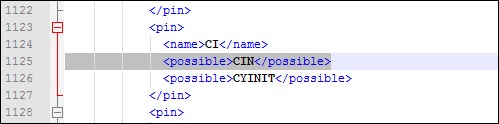
\includegraphics[width=.9\columnwidth]{cellLibHandEdit.png}
  \end{figure}
  
  You should have to insert this line in two places only.
  \item Save your changes and exit the text editor
  \item Copy the XML file to \textit{RapidSmithPath/device/family}
  directory where ``family'' is replaced by the family of your part (such as
  artix7), and ``RapidSmithPath'' is the location of your RapidSmith repository.
  Once this is complete the new \cls{CellLibrary} should be ready to use. 
\end{enumerate}

\pgm{NOTE}: Parts in the same family can usually use the same
\cls{CellLibrary}.
